\documentclass[12pt, %
openright, 
oneside, %
%twoside, %TCC: Se seu texto tem mais de 100 páginas, descomente esta linha e comente a anterior
a4paper,    %
%english,   %
brazil]{facom-ufu-abntex2}

\usepackage{graphicx}
\graphicspath{{figuras/}{pictures/}{images/}{./}} % where to search for the images

\newcommand{\blue}[1]{\textcolor{blue}{#1}}
\newcommand{\red}[1]{\textcolor{red}{#1}}


\autor{Daniel Gonçalves - 12011BCC011 , João Victor Fernandes de Souza Silva - 11911BSI205, Luiz André de Silva Carvalho - 11911BSI225} %TCC %TCC
%\coorientador{Algum?} %TCC

% ---
% Informações de dados para CAPA e FOLHA DE ROSTO
% ---

\titulo{ Implementação de um perceptron para classificar dados da base Iris} %TCC

\begin{document} 
\frenchspacing 

% ----------------------------------------------------------
% ELEMENTOS PRÉ-TEXTUAIS
% ----------------------------------------------------------
%\pretextual
\imprimircapa


%%As seções dedicatória, agradecimento e epígrafe não são obrigatórias.
%%Só as mantenha se achar pertinente.

% ---
% Dedicatória
% ---
%\begin{dedicatoria}
%   \vspace*{\fill}
%   \centering
%   \noindent
%   \textit{Dedico a \lipsum[10]}  %TCC:
%   \vspace*{\fill}
%\end{dedicatoria}
% ---

% ---
% Agradecimentos
% ---
%\begin{agradecimentos}
%Agradeço a \lipsum[30]. %TCC:
%\end{agradecimentos}
% ---

% ---
% Epígrafe
% ---
%\begin{epigrafe}
%    \vspace*{\fill}
%	\begin{flushright}
%		\textit{``Alguma citação que ache conveniente? \lipsum[10]''} %TCC:
%	\end{flushright}
%\end{epigrafe}
% ---


% ---
% inserir lista de ilustrações
% ---
\pdfbookmark[0]{\listfigurename}{lof}
\listoffigures*
\cleardoublepage
% ---

\chapter{Introdução}
O presente relatório se refere à implementação de um Perceptron para a classificação de duas espécies da base de flores Iris. Diferentes valores para os parâmetros de taxa de aprendizado, épocas e proporção da base usada para o treinamento foram considerados. Além disso, foram realizados experimentos considerando as diversas combinações das 3 espécies disponíveis, com a terceira sendo aplicada sobre o modelo já treinado e o resultado analisado.

\chapter{Implementação}
O Perceptron foi implementado na linguagem de programação Python. Instruções para instalação das bibliotecas necessárias e como executar o programa estão disponíveis no README do projeto.

\section{Dados de entrada}
Dadas as duas espécies que serão usadas para o treinamento do neurônio a primeira etapa realizada é a normalização dos dados por meio da técnica min-max. A normalização é aplicada nos dados de todas as três espécies, mas o MIN e o MAX são calculados apenas das duas espécies escolhidas.

\section{Classe Perceptron}
Uma classe foi criada para conter os métodos e as variáveis associadas ao Perceptron. Os pesos (incluindo o bias) são armazenados em um vetor de Floats, o qual é inicializado aleatoriamente com números entre -1 e 1 assim que o objeto da classe é criado.

\section{Função de Ativação}
Para este trabalho simples escolhemos a função de ativação sigmóide. Caso seu retorna seja menor ou igual que 0.5 o neurônio classifica como a primeira espécie passado, e se for maior que 0.5 classifica como a segunda espécie.

\chapter{Testes e Resultados}
Para as realizações dos testes, foram escolhidas as classes Setosa e Virginica. Abaixo são demonstrados os testes com os seus respectivos resultados levando em consideração variações para os valores da taxa de aprendizado, total de iterações e três conjuntos de treino: Iris10, Iris30 e Iris50. Cada conjunto de treino pode ser definido, respectivamente como 10\%, 30\% e 50\% da base de dados Iris.

\section{Testes e resultados para o conjunto de dados Iris10}
Para todos os testes, foi considerado um valor constante do total de iterações sendo 20 e variações da taxa de aprendizado.

Para o primeiro teste, com uma taxa de aprendizado de 10\%. A acurácia obtida foi de 97.77\% sendo possível observar a variação da acurácia em relação ao conjunto de dados normalizado pela figura \ref{fig:1} e a variação de erro por epoch pela figura \ref{fig:2}.

\begin{figure}[H]
\centering
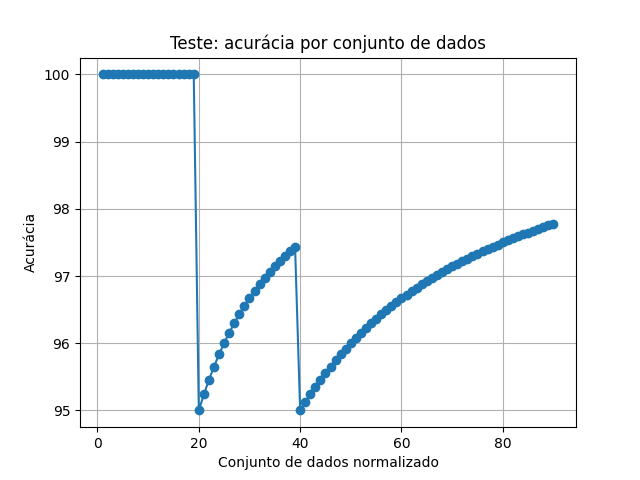
\includegraphics[scale=0.9]{figuras/acuracia1.png}
\caption{Base Iris10 - relação entre acurácia e conjunto de dados normalizado para taxa de aprendizado de 10\%}
\label{fig:1}
\end{figure}

\begin{figure}[H]
\centering
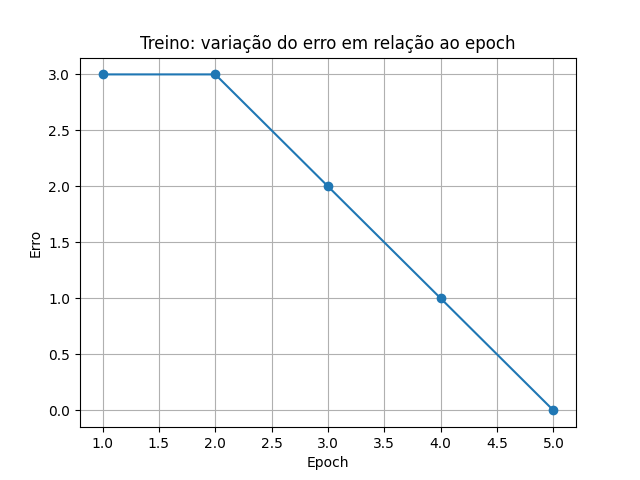
\includegraphics[scale=0.9]{figuras/erro1.png}
\caption{Base Iris10 - relação entre erro e epoch para taxa de aprendizado de 10\%}
\label{fig:2}
\end{figure}

Já para o segundo teste, com uma taxa de aprendizado de 20\%. A acurácia obtida foi de 84.44\% sendo possível observar a variação da acurácia em relação ao conjunto de dados normalizado pela figura \ref{fig:3} e a variação de erro por epoch pela figura \ref{fig:4}.

\begin{figure}[H]
\centering
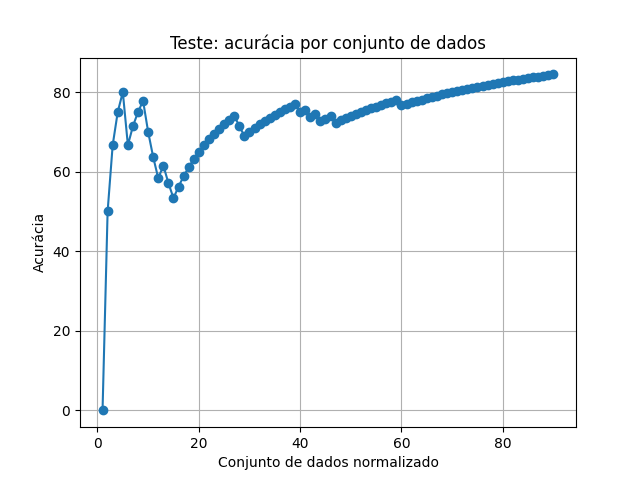
\includegraphics[scale=0.9]{figuras/acuracia_2.png}
\caption{Base Iris10 - relação entre acurácia e conjunto de dados normalizado para taxa de aprendizado de 20\%}
\label{fig:3}
\end{figure}
\begin{figure}[H]
\centering
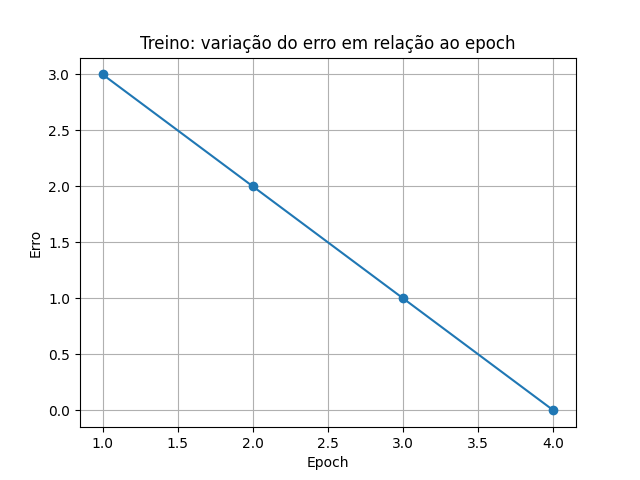
\includegraphics[scale=0.9]{figuras/erro_2.png}
\caption{Base Iris10 - relação entre erro e epoch para taxa de aprendizado de 20\%}
\label{fig:4}
\end{figure}

Por último, foi considerado uma taxa de aprendizado de 30\%. A acurácia obtida foi de 86.66\% sendo possível observar a variação da acurácia em relação ao conjunto de dados normalizado pela figura \ref{fig:5} e a variação de erro por epoch pela figura \ref{fig:6}.

\begin{figure}[H]
\centering
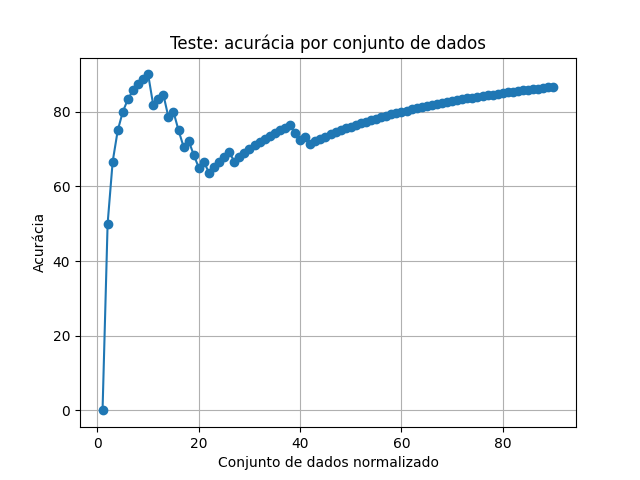
\includegraphics[scale=0.9]{figuras/acuracia_3.png}
\caption{Base Iris10 - relação entre acurácia e conjunto de dados normalizado para taxa de aprendizado de 30\%}
\label{fig:5}
\end{figure}

\begin{figure}[H]
\centering
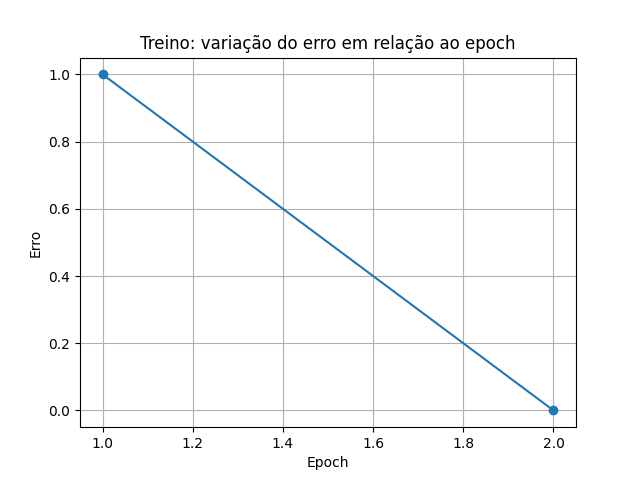
\includegraphics[scale=0.9]{figuras/erro_3.png}
\caption{Base Iris10 - relação entre erro e epoch para taxa de aprendizado de 30\%}
\label{fig:6}
\end{figure}

Portanto, tais oscilações no valor da acurácia deve-se ao tamanho da base e a forma como a taxa de aprendizagem afeta no treinamento, visto que quanto menor a taxa de aprendizagem, menos ajustes nos pesos serão realizados pelo modelo a cada iteração, explicando assim a maior acurácia para quando a taxa de aprendizagem é de 10\%.

\section{Testes e resultados para o conjunto de dados Iris30}
Para todos os testes, foi considerado um valor constante do total de iterações sendo 50 e variações da taxa de aprendizado.

Para o primeiro teste, com uma taxa de aprendizado de 10\%. A acurácia obtida foi de 94.28\% sendo possível observar a variação da acurácia em relação ao conjunto de dados normalizado pela figura \ref{fig:7} e a variação de erro por epoch pela figura \ref{fig:8}.

\begin{figure}[H]
\centering
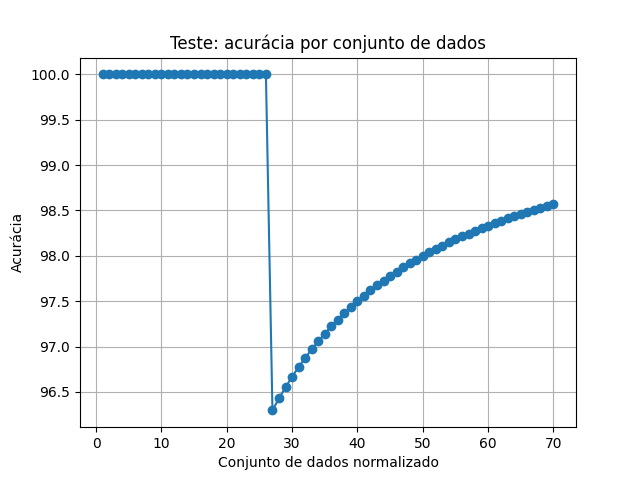
\includegraphics[scale=0.9]{figuras/acuracia_4.png}
\caption{Base Iris30 - relação entre acurácia e conjunto de dados normalizado para taxa de aprendizado de 10\%}
\label{fig:7}
\end{figure}

\begin{figure}[H]
\centering
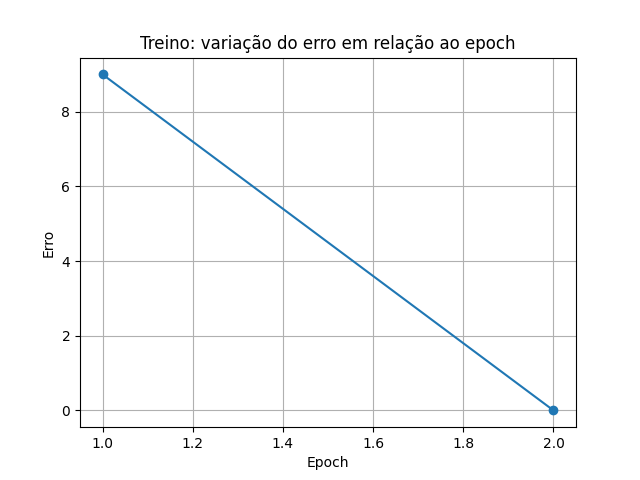
\includegraphics[scale=0.9]{figuras/erro_4.png}
\caption{Base Iris30 - relação entre erro e epoch para taxa de aprendizado de 10\%}
\label{fig:8}
\end{figure}

Já para o segundo teste, com uma taxa de aprendizado de 20\%. A acurácia obtida foi de 97.14\% sendo possível observar a variação da acurácia em relação ao conjunto de dados normalizado pela figura \ref{fig:9} e a variação de erro por epoch pela figura \ref{fig:10}.

\begin{figure}[H]
\centering
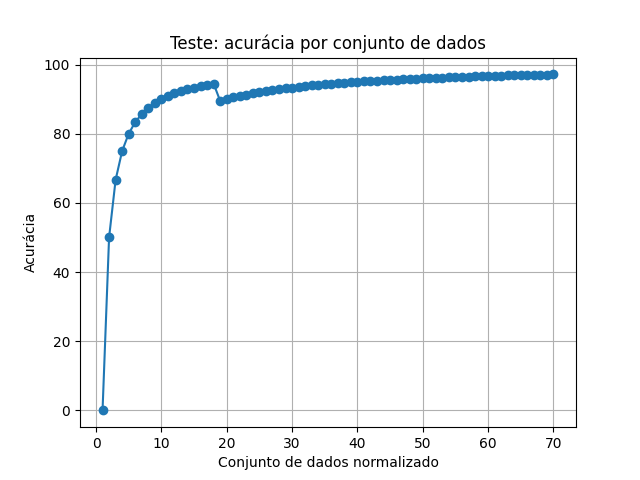
\includegraphics[scale=0.9]{figuras/acuracia_5.png}
\caption{Base Iris30 - relação entre acurácia e conjunto de dados normalizado para taxa de aprendizado de 20\%}
\label{fig:9}
\end{figure}

\begin{figure}[H]
\centering
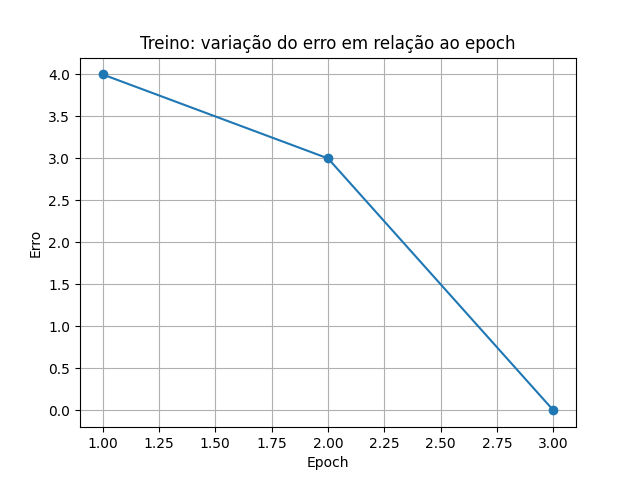
\includegraphics[scale=0.9]{figuras/erro_5.png}
\caption{Base Iris30 - relação entre erro e epoch para taxa de aprendizado de 20\%}
\label{fig:10}
\end{figure}

Por último, foi considerado uma taxa de aprendizado de 30\%. A acurácia obtida foi de 98.57\% sendo possível observar a variação da acurácia em relação ao conjunto de dados normalizado pela figura \ref{fig:11} e a variação de erro por epoch pela figura \ref{fig:12}.

\begin{figure}[H]
\centering
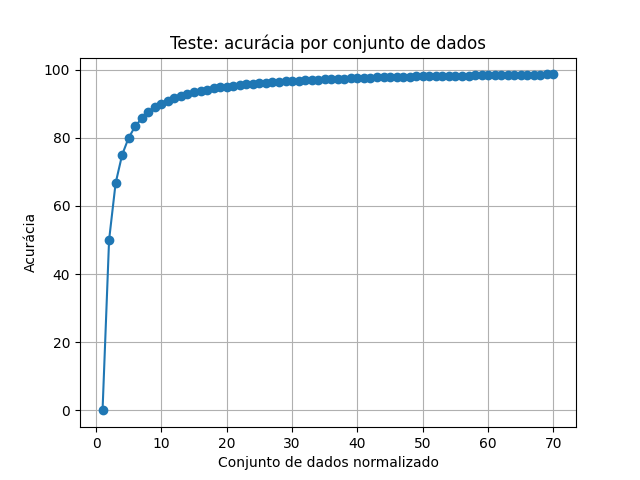
\includegraphics[scale=0.9]{figuras/acuracia_6.png}
\caption{Base Iris30 - relação entre acurácia e conjunto de dados normalizado para taxa de aprendizado de 30\%}
\label{fig:11}
\end{figure}

\begin{figure}[H]
\centering
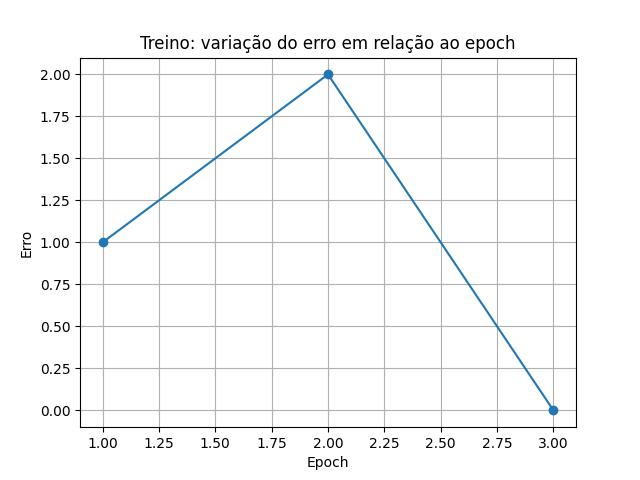
\includegraphics[scale=0.9]{figuras/erro_6.png}
\caption{Base Iris30 - relação entre erro e epoch para taxa de aprendizado de 30\%}
\label{fig:12}
\end{figure}

Assim, é possível concluir que a alteção do tamanho do conjunto de dados afetou a acurácia consideravelmente quando comparado aos resultados obtidos nos testes realizados com a base Iris10, além também das variações da taxa de aprendizagem e épocas. Logo, uma maior quantidade de dados ajuda o modelo a aprender padrões mais robustos e a generalizar melhor. 

\section{Testes e resultados para o conjunto de dados Iris50}
Para todos os testes, foi considerado um valor constante do total de iterações sendo 10 e variações da taxa de aprendizado.

Para o primeiro teste, com uma taxa de aprendizado de 10\%. A acurácia obtida foi de 98\% sendo possível observar a variação da acurácia em relação ao conjunto de dados normalizado pela figura \ref{fig:13} e a variação de erro por epoch pela figura \ref{fig:14}.

\begin{figure}[H]
\centering
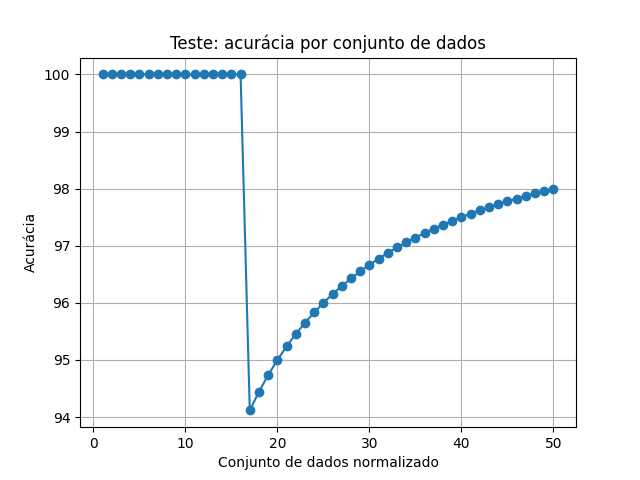
\includegraphics[scale=0.9]{figuras/acuracia_7.png}
\caption{Base Iris50 - relação entre acurácia e conjunto de dados normalizado para taxa de aprendizado de 10\%}
\label{fig:13}
\end{figure}

\begin{figure}[H]
\centering
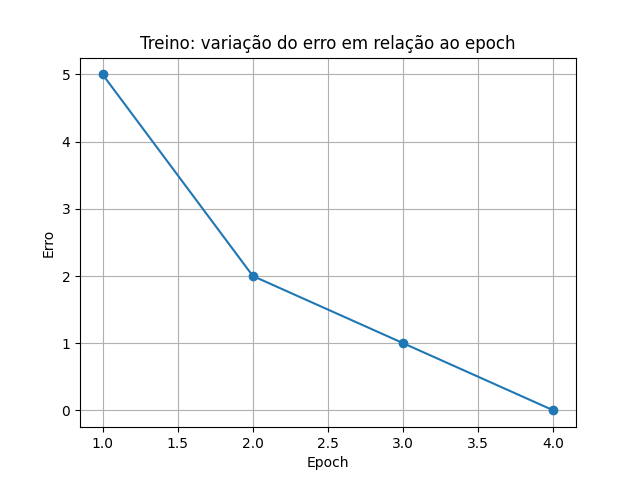
\includegraphics[scale=0.9]{figuras/erro_7.png}
\caption{Base Iris50 - relação entre erro e epoch para taxa de aprendizado de 10\%}
\label{fig:14}
\end{figure}

Já para o segundo teste, com uma taxa de aprendizado de 20\%. A acurácia obtida foi de 98\% sendo possível observar a variação da acurácia em relação ao conjunto de dados normalizado pela figura \ref{fig:15} e a variação de erro por epoch pela figura \ref{fig:16}.

\begin{figure}[H]
\centering
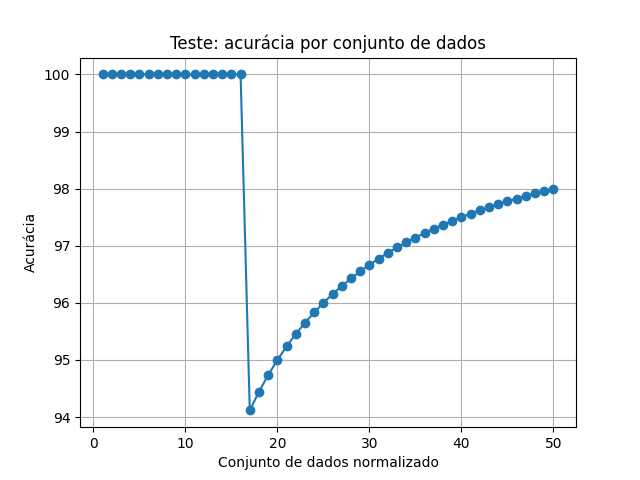
\includegraphics[scale=0.9]{figuras/acuracia_8.png}
\caption{Base Iris50 - relação entre acurácia e conjunto de dados normalizado para taxa de aprendizado de 20\%}
\label{fig:15}
\end{figure}

\begin{figure}[H]
\centering
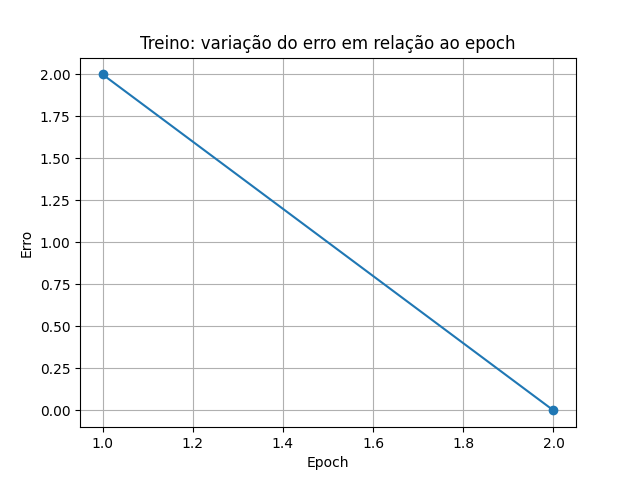
\includegraphics[scale=0.9]{figuras/erro_8.png}
\caption{Base Iris50 - relação entre erro e epoch para taxa de aprendizado de 20\%}
\label{fig:16}
\end{figure}

Por último, foi considerado uma taxa de aprendizado de 30\%. A acurácia obtida foi de 98\% sendo possível observar a variação da acurácia em relação ao conjunto de dados normalizado pela figura \ref{fig:17} e a variação de erro por epoch pela figura \ref{fig:18}.

\begin{figure}[H]
\centering
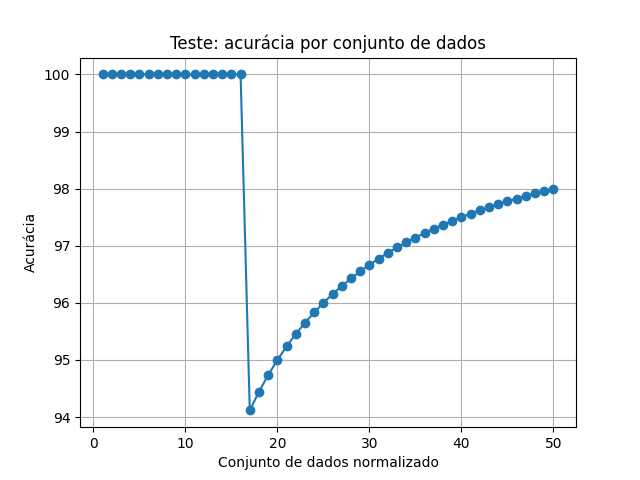
\includegraphics[scale=0.9]{figuras/acuracia_9.png}
\caption{Base Iris50 - relação entre acurácia e conjunto de dados normalizado para taxa de aprendizado de 30\%}
\label{fig:17}
\end{figure}

\begin{figure}[H]
\centering
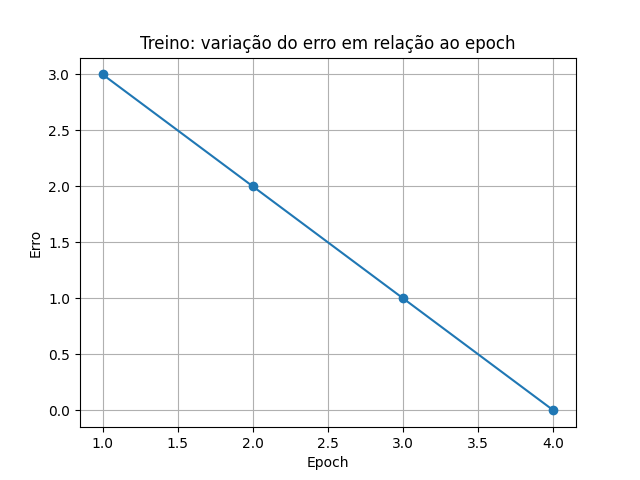
\includegraphics[scale=0.9]{figuras/erro_9.png}
\caption{Base Iris50 - relação entre erro e epoch para taxa de aprendizado de 30\%}
\label{fig:18}
\end{figure}

Sendo assim, é possível concluir que com um base de 50\% obtém-se dados altamente informativos e bem distribuídos implicando assim em uma acurácia constante independete da taxa de aprendizagem.

\section{Teste e resultados para inserção da terceira classe}
Ao inserir a terceira classe(Versicolour), com exceção dos testes realizados com a base de treino Iris10 onde foram obtidos 44 registros classificados como Virginica e 6 como Sentosa para a taxa de aprendizagem de 10\% e 43 registros classificados como Virginica e 7 como Sentosa para a taxa de aprendizagem de 20\%, toda a base para a classe Versicolour foi classificada como Virginica, o motivo desta classificação pode ser observado na figura \ref{fig:19}. Tal classificação se dá devido as características em comum entre as duas classes.
\begin{figure}[H]
\centering
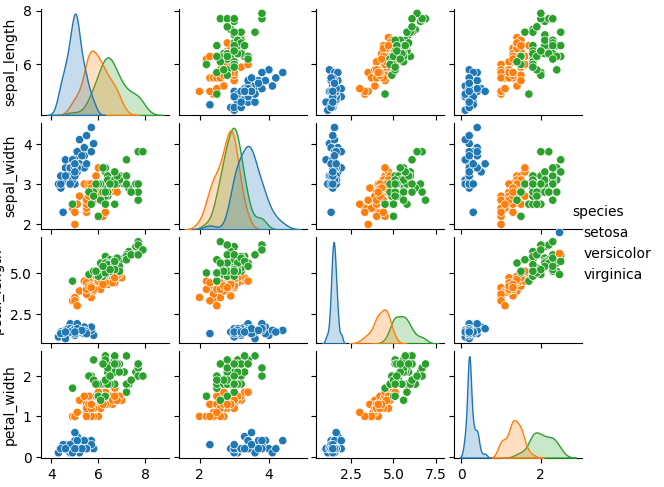
\includegraphics[scale=0.9]{figuras/base_iris.png}
\caption{Iris: características das flores e suas espécies}
\label{fig:19}
\end{figure}

\end{document}